\thispagestyle{plain}
{\tabcolsep=0pt
\noindent
\begin{tabular}{>{\centering}p{11cm}}
\includegraphics[scale=0.82]{figures/01.png}\\
\textbf{ ಶ್ರೀಯುತರು ಅಧ್ಯಯನ ಮತ್ತು ಅಧ್ಯಾಪನ ಮಾಡಿದ\\ ಮಹಾರಾಜಸಂಸ್ಕೃತ ಮಹಾಪಾಠಶಾಲೆ, ಮೈಸೂರು.}\\[12pt]
\includegraphics[scale=0.85]{figures/02.png}\\
\textbf{ ಶ್ರೀಯುತರು ಅಧ್ಯಯನ ಮತ್ತು ಅಧ್ಯಾಪನ ಮಾಡಿದ ಮಹಾರಾಜಸಂಸ್ಕೃತ\\ ಮಹಾಪಾಠಶಾಲೆಯ ಇನ್ನೊಂದು ನೋಟ}
\end{tabular}
}

\eject
\thispagestyle{plain}

{\tabcolsep=0pt
\noindent
\begin{tabular}{>{\centering}p{11cm}}
\includegraphics{figures/03.png}\\
\textbf{ಮಹಾರಾಜಸಂಸ್ಕೃತಮಹಾ ಪಾಠಶಾಲೆಯ ಮಹಾದ್ವಾರ}\\[15pt]
\includegraphics[scale=0.9]{figures/05.png}\\
\textbf{ಪಾಠಶಾಲೆಯ ಸರಸ್ವತೀಪ್ರಾಸಾದದಲ್ಲಿರುವ ವಿದ್ಯಾಗಣಪತಿ ಮಹಾಸನ್ನಿಧಾನ}
\end{tabular}
}

\eject
\thispagestyle{plain}

{\tabcolsep=0pt
\noindent
\begin{tabular}{>{\centering}p{11cm}}
\includegraphics[scale=0.95]{figures/06.png}\\
\textbf{ ಶ್ರೀಯುತರನ್ನು ಬರಮಾಡಿಕೊಳ್ಳಲು ದ್ವಾರದಲ್ಲಿ ಕಾತರಿಸುತ್ತಿರುವ  ಶಿಷ್ಯವೃಂದ}\\[12pt]
\includegraphics[scale=0.95]{figures/08.png}\\
\textbf{ವಾಹನದಲ್ಲಿ ಶ್ರೀಯುತರ ಆಗಮನ}\\[12pt]
\includegraphics[scale=0.95]{figures/09.png}\\
\textbf{ಪೂರ್ಣಕುಂಭಸ್ವಾಗತ}
\end{tabular}
}

\eject
\thispagestyle{plain}

{\tabcolsep=0pt
\noindent
\begin{tabular}{>{\centering}p{11cm}}
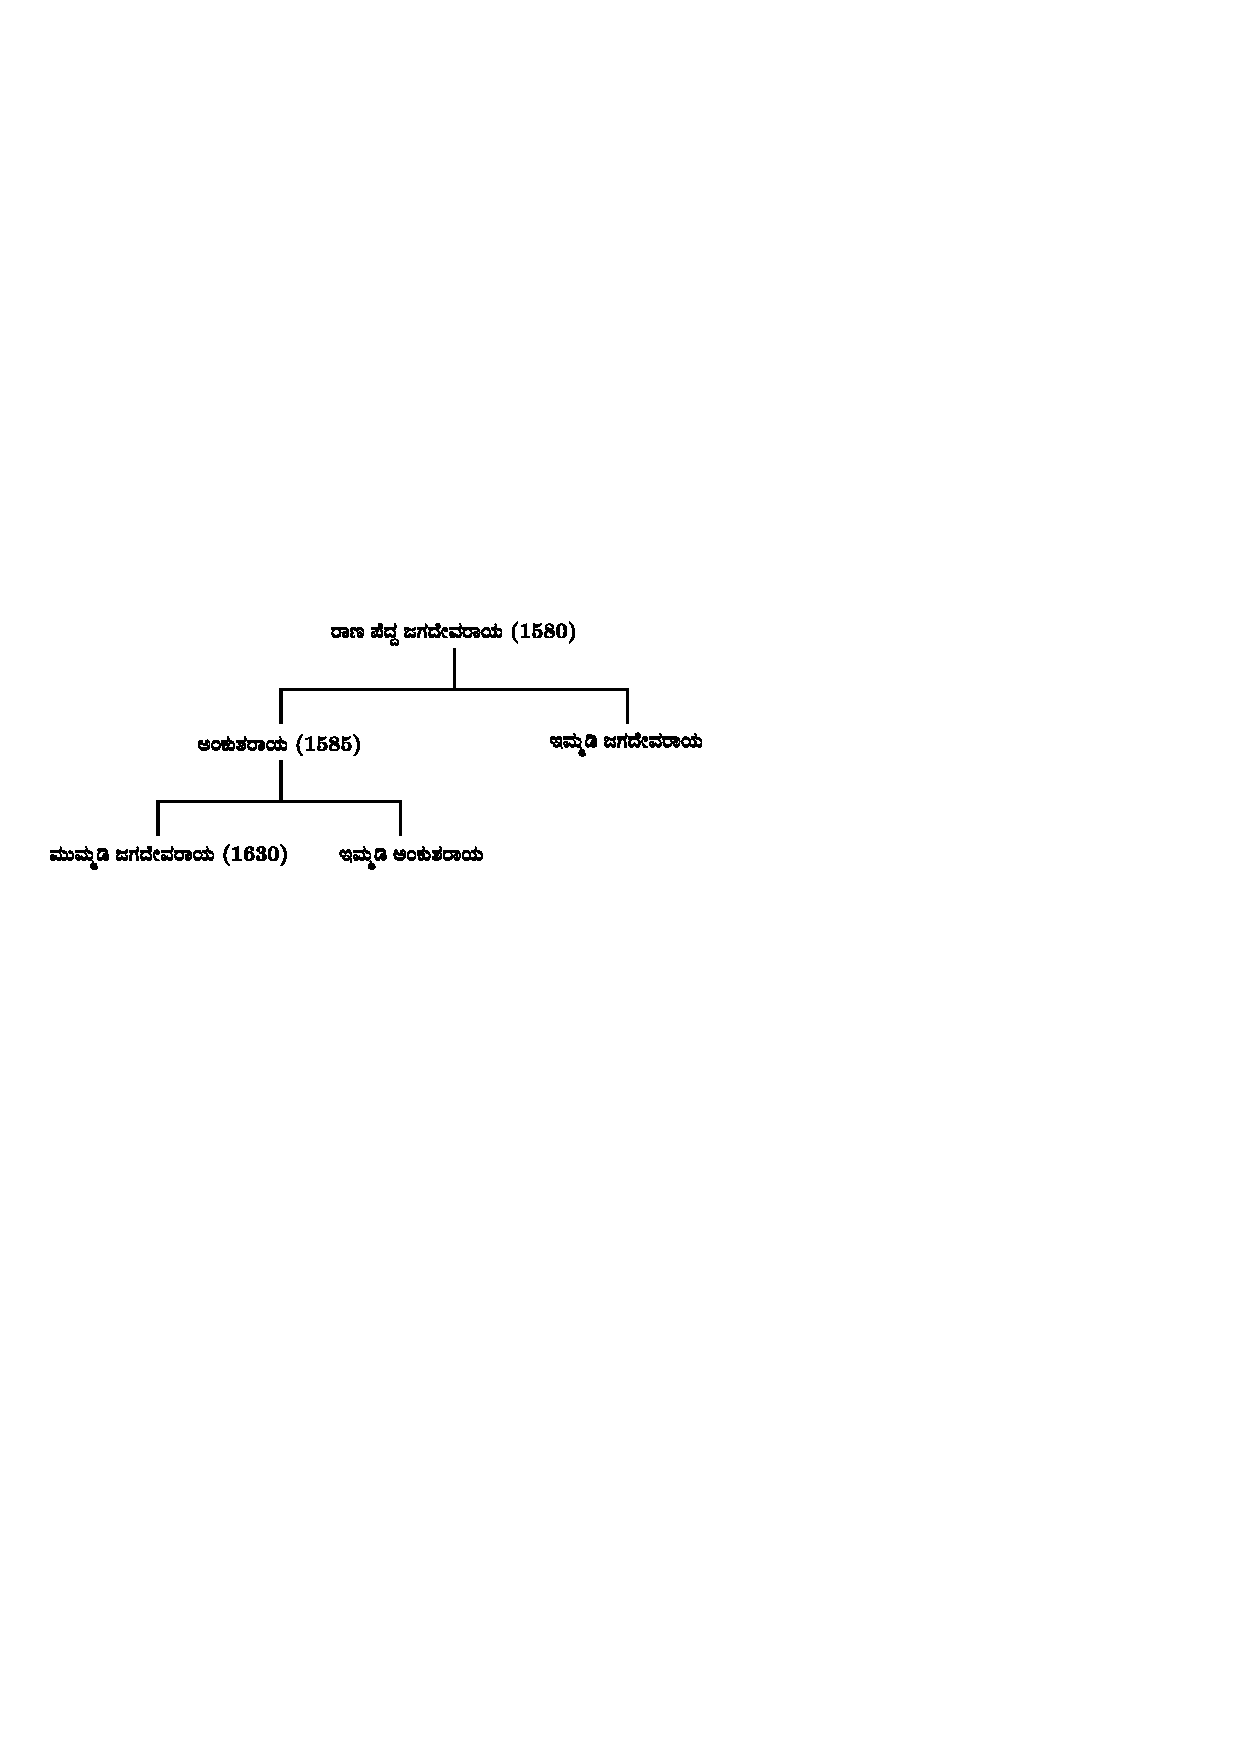
\includegraphics[scale=0.95]{figures/10.png}\\
\textbf{ವೇದಸ್ವಸ್ತಿಯೊದಿಗೆ ಶುಭಾಗಮನ}\\[12pt]
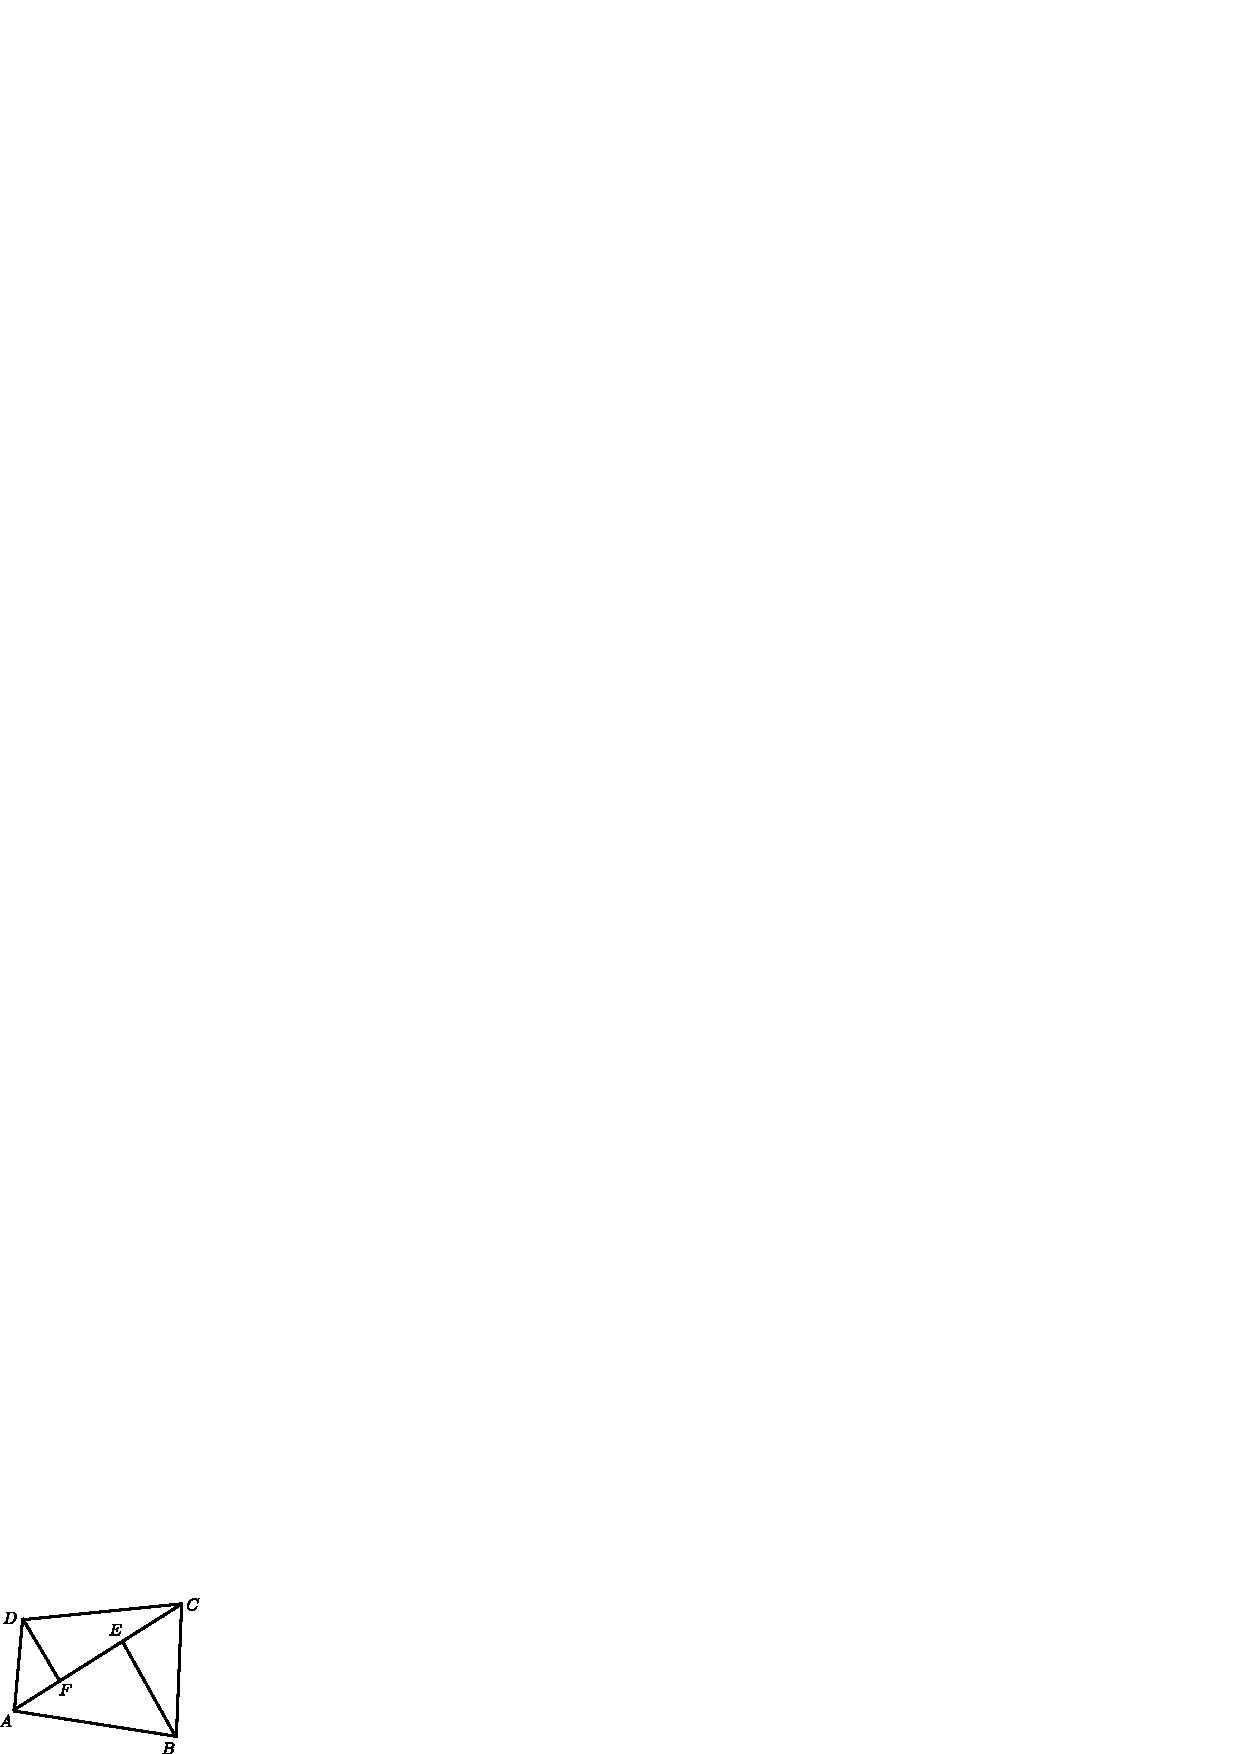
\includegraphics[scale=0.95]{figures/11.png}\\
\textbf{ಗಣಪತಿ ಅರ್ಚಕರಿಂದ ಆಶೀರ್ವಾದ}\\[12pt]
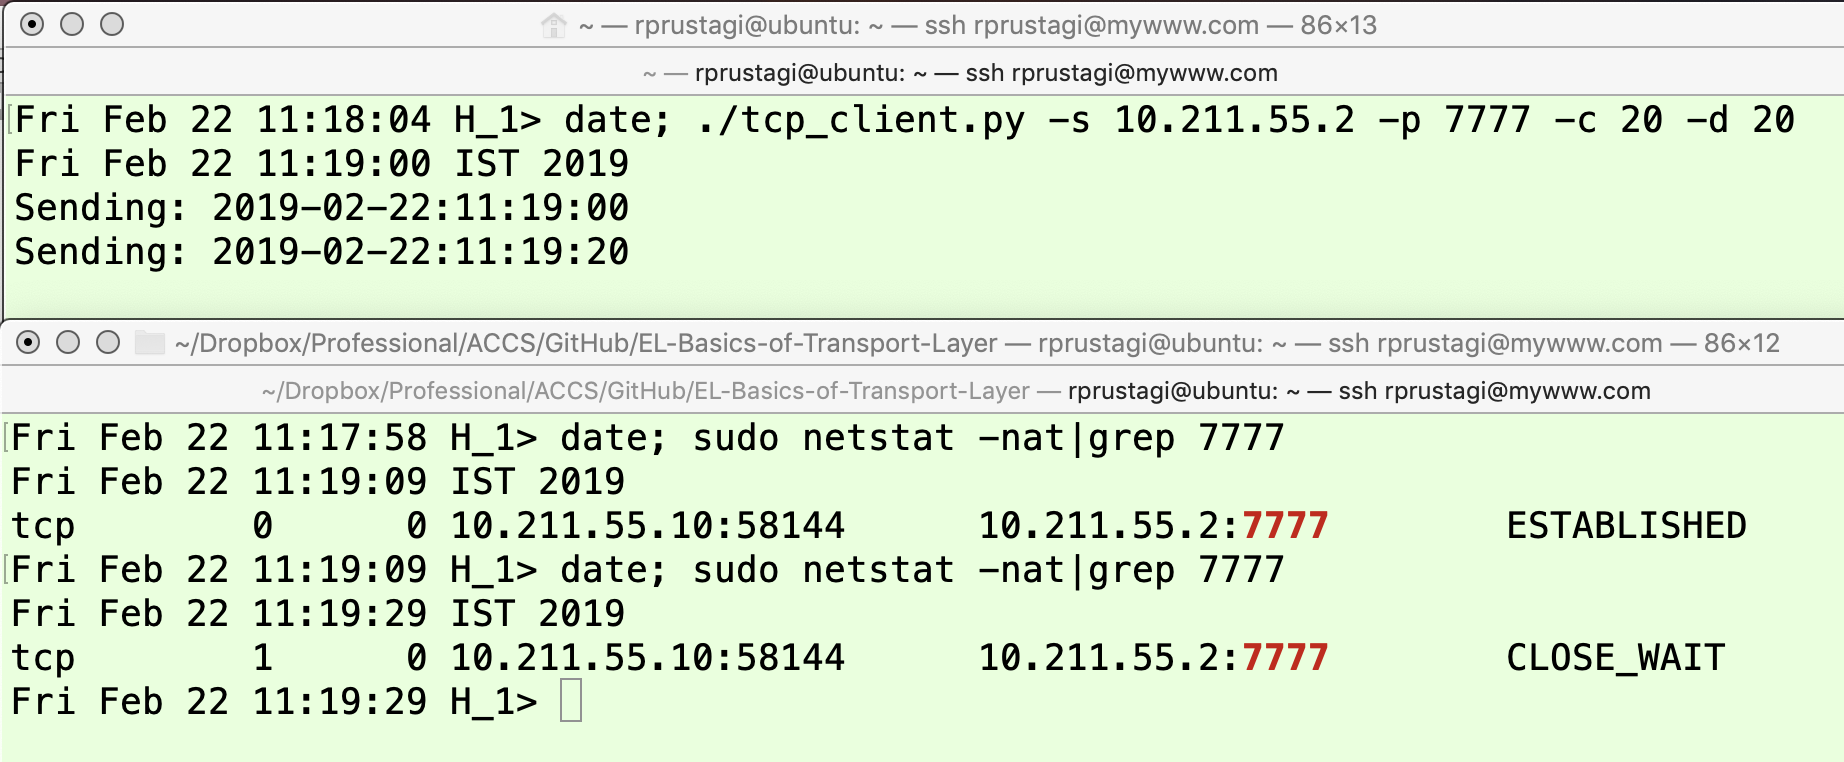
\includegraphics[scale=0.95]{figures/12.png}\\
\textbf{ದೀಪಪ್ರಜ್ವಾಲನಪೂರ್ವಕ ಕಾರ್ಯಕ್ರಮದ ಉದ್ಘಾಟನೆ- ರಜೇಶ್ವರಶಾಸ್ತ್ರಿಗಳಿಂದ}
\end{tabular}
}

\eject
\thispagestyle{plain}

{\tabcolsep=0pt
\noindent
\begin{tabular}{>{\centering}p{11cm}}
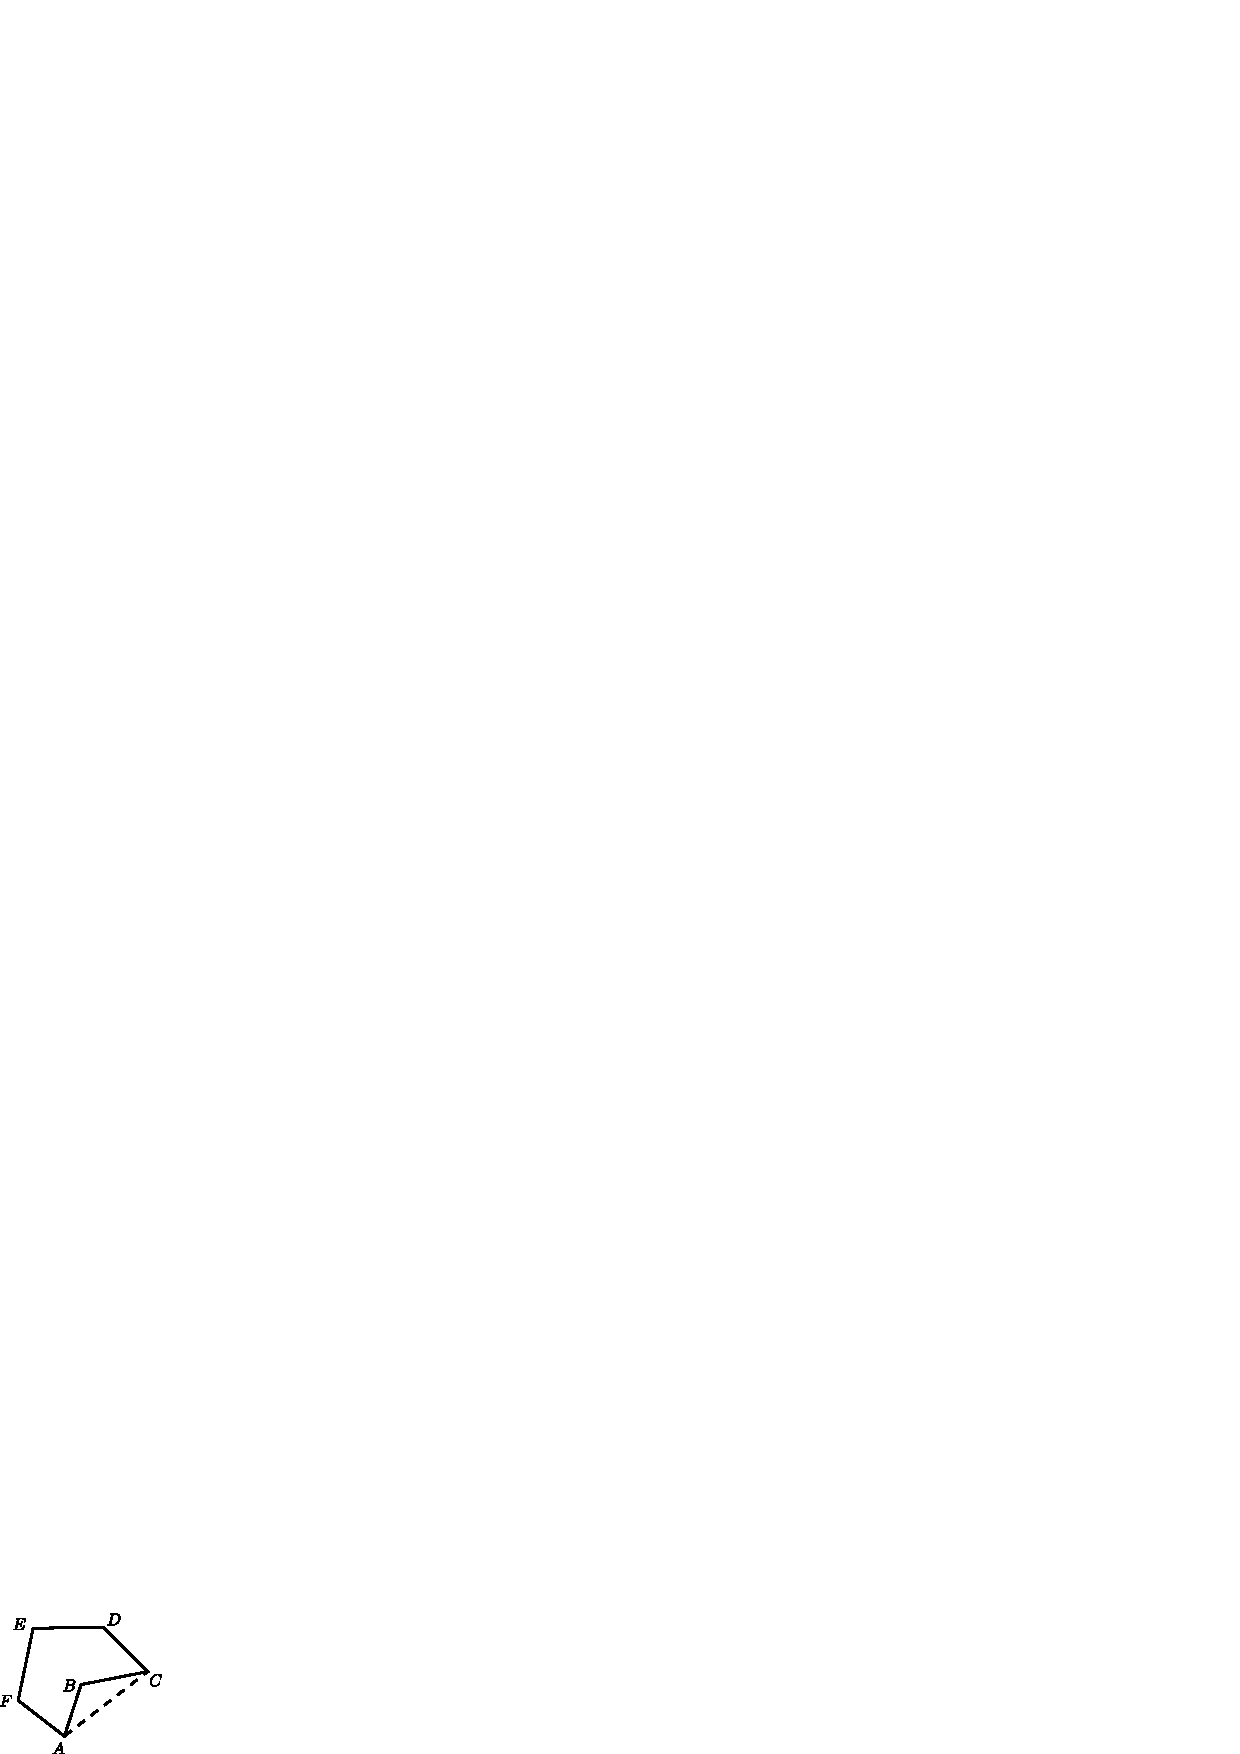
\includegraphics[scale=0.9]{figures/13.png}\\
\textbf{ಭಟ್ಟರಿಗೆ ಸಮರ್ಪಿಸಲು  ಸಿದ್ಧಗಪಡಿಸಿರುವ ಶ್ರ್ಶ್ರೀಯುತರಾಮಭದ್ರಾಚಾರ್ಯ\\ ದಂಪತಿಗಳ ಭಾವಚಿತ್ರ}\\[12pt]
\includegraphics[scale=0.9]{figures/13a.png}\\
\textbf{ದೀಪಪ್ರಜ್ವಾಲಪೂರ್ವಕ ಕಾರ್ಯಕ್ರಮದ ಉದ್ಘಾಟನೆ - ಗಂಗಾಧರ ಭಟ್ಟರಿಂದ}\\[12pt]
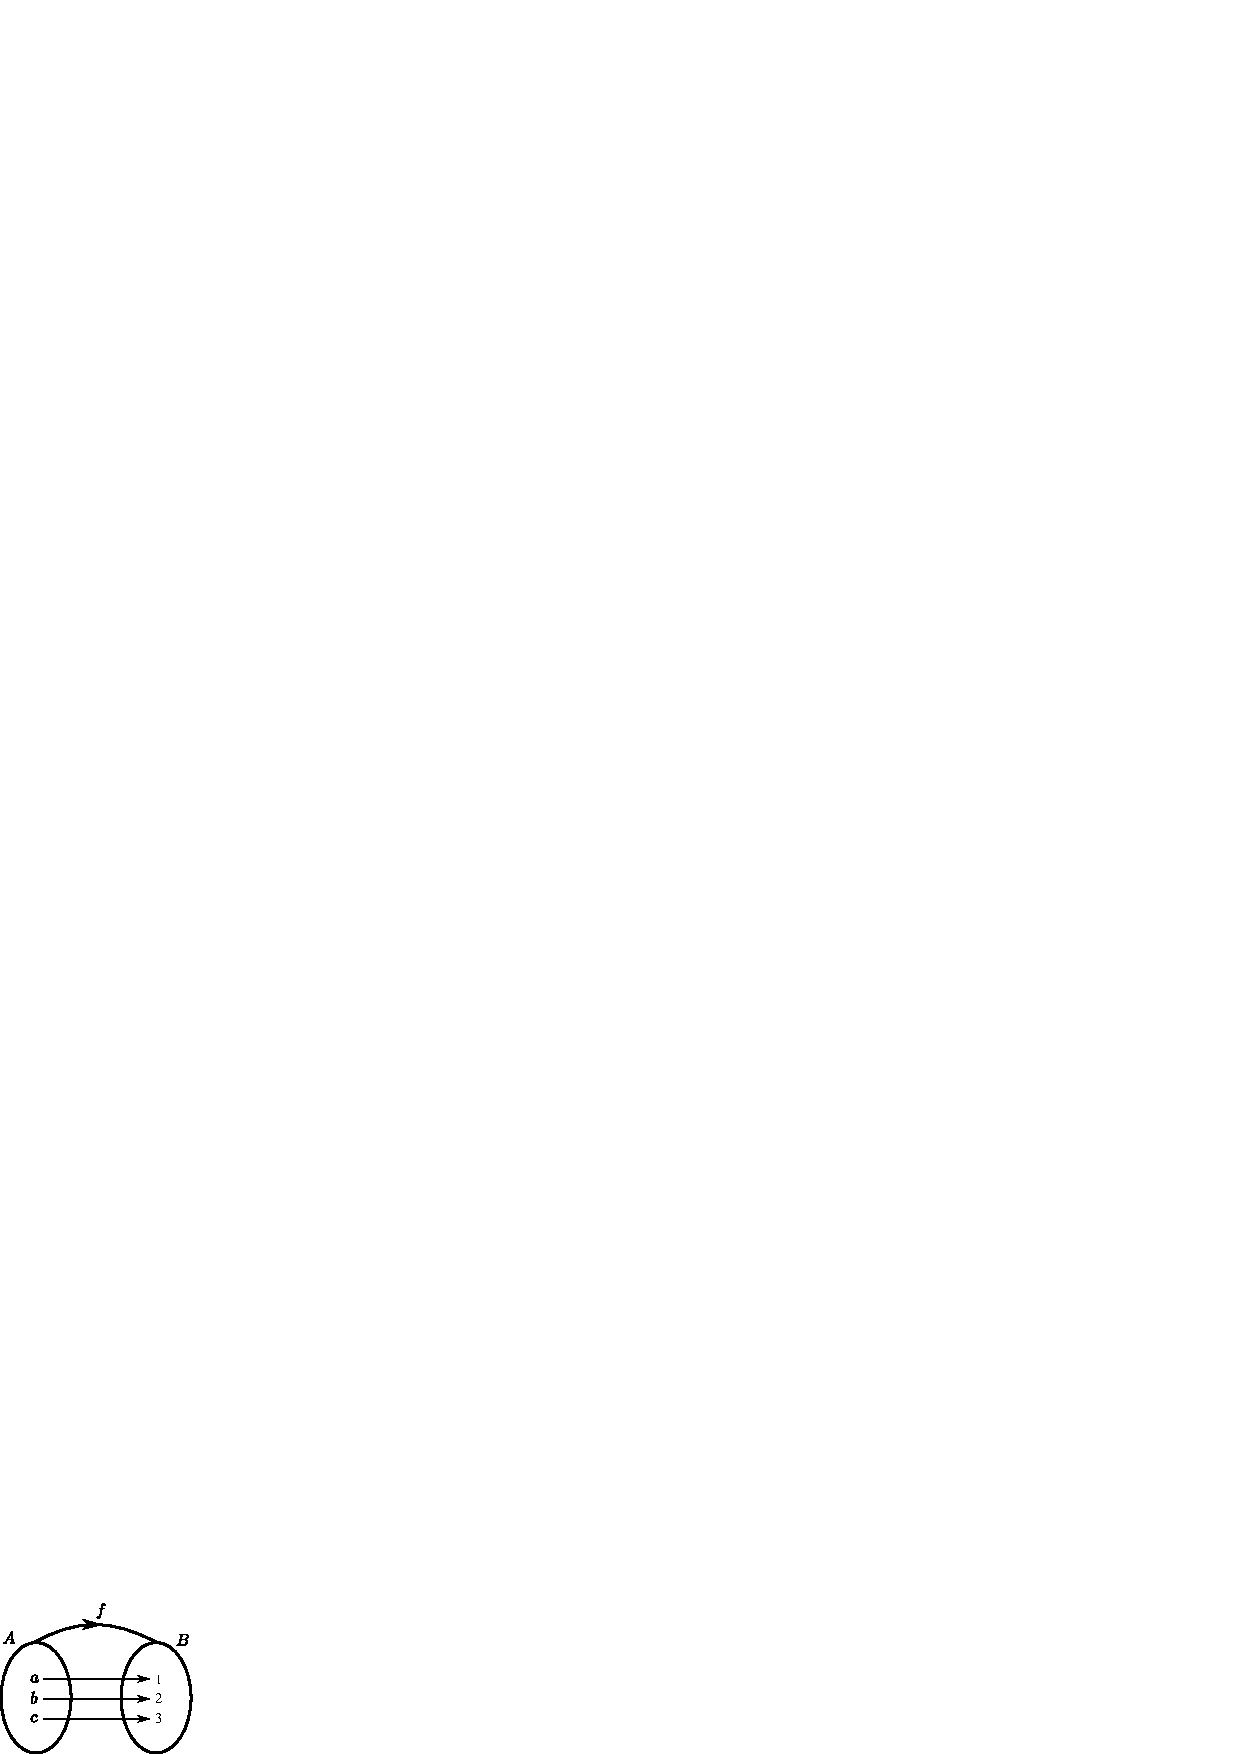
\includegraphics[scale=0.9]{figures/14.png}\\
\textbf{ವಾಕ್ಯಾರ್ಥಗೋಷ್ಠಿಯಲ್ಲಿ ಮಂದಿಸಿರುವ ವಿದ್ವಾಂಸರು}
\end{tabular}
}

\eject
\thispagestyle{plain}

{\tabcolsep=0pt
\noindent
\begin{tabular}{>{\centering}p{11cm}}
\includegraphics[scale=0.95]{figures/14a.png}\\
\textbf{ವಾಕ್ಯಾರ್ಥಗೋಷ್ಠೀ ಸಂದರ್ಭ}\\[12pt]
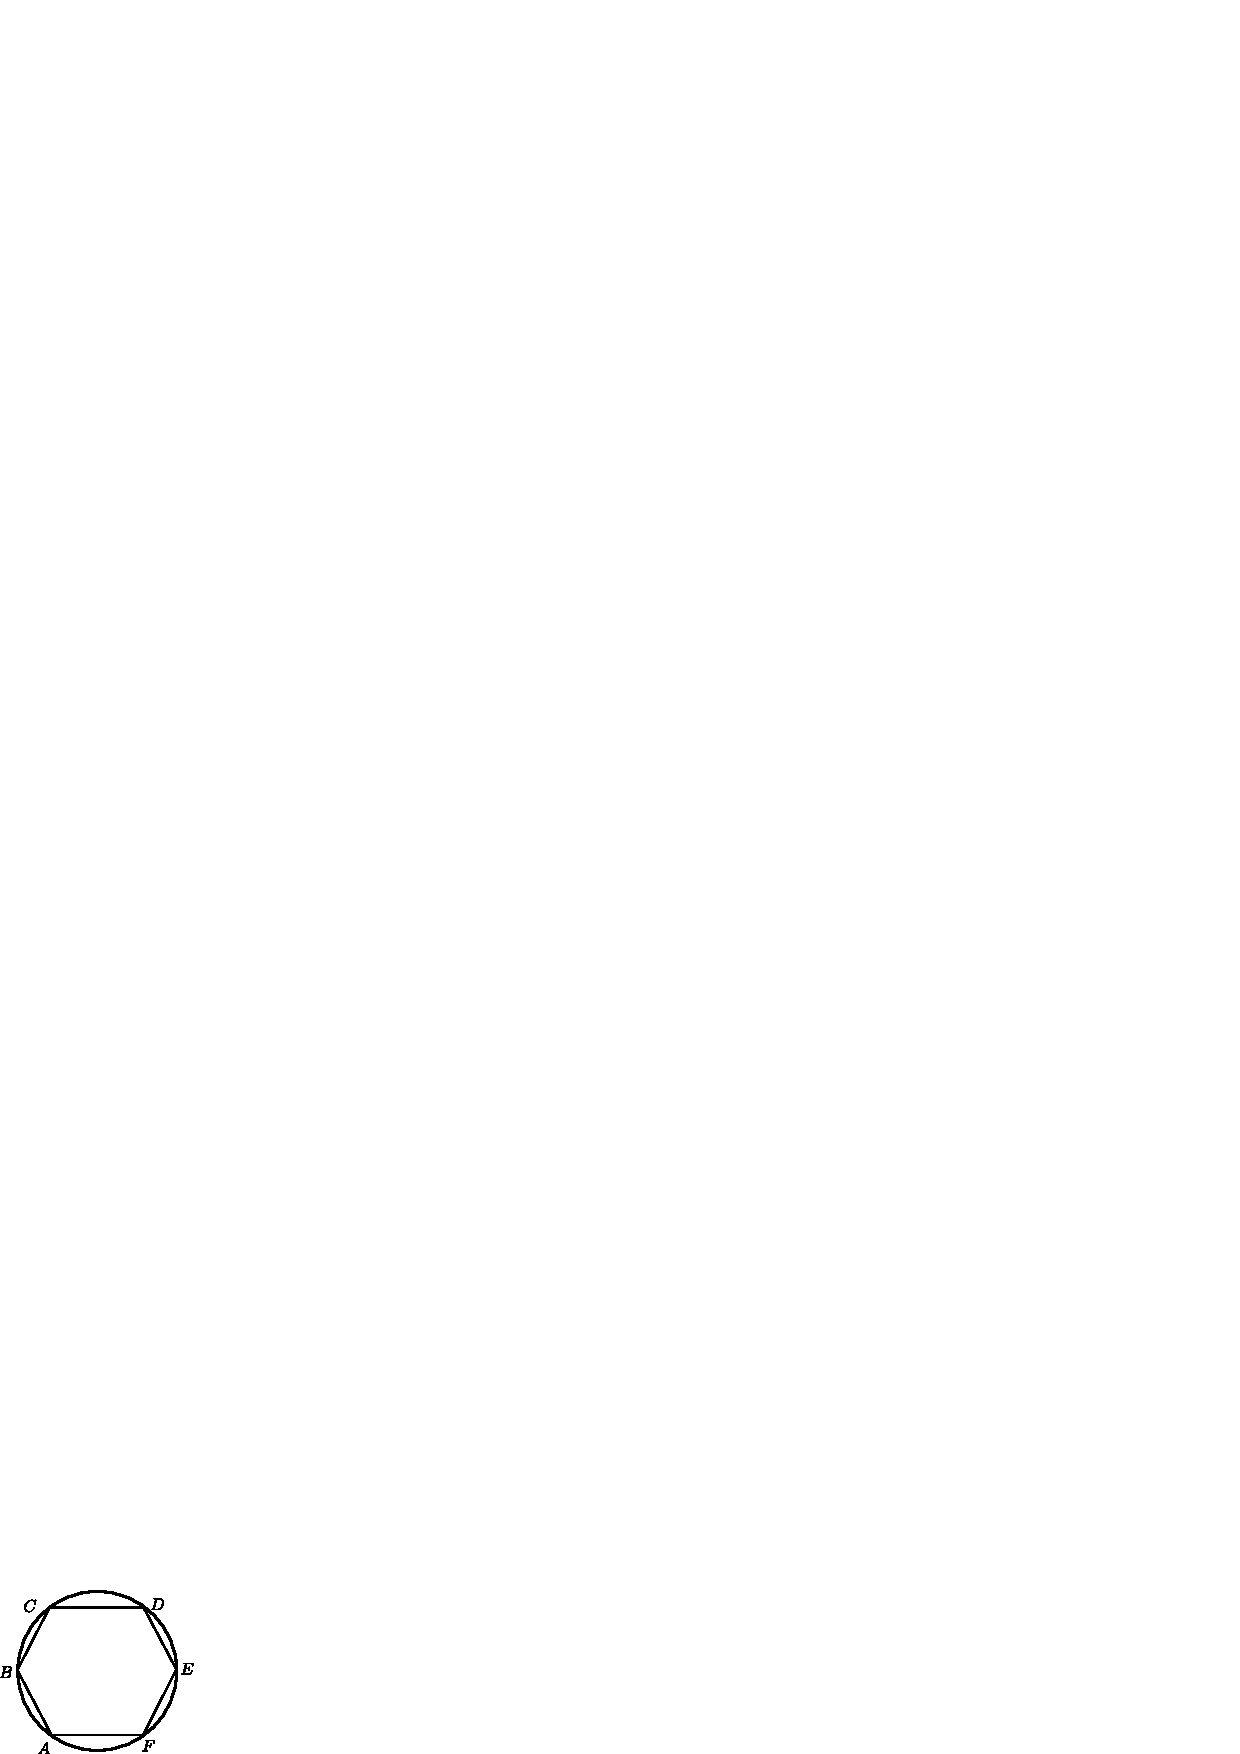
\includegraphics[scale=0.95]{figures/15.png}\\
\textbf{ಗಂಗಾಧರ ಭಟ್ಟರ ವಿದ್ಯಾರ್ಥಿ ಶ್ರೀಶಿವರಾಮರಿಂದ ವಾಖ್ಯಾರ್ಥ}\\[12pt]
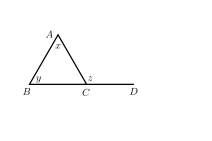
\includegraphics[scale=0.95]{figures/16.png}\\
\textbf{ಗಂಗಾಧರ ಭಟ್ಟರ ವಿದ್ಯಾರ್ಥಿ ಶ್ರೀ ಕೆ ಎಲ್ ರಾಘವರಿಂದ ವಾಖ್ಯಾರ್ಥ}
\end{tabular}
}

\eject
\thispagestyle{plain}

{\tabcolsep=0pt
\noindent
\begin{tabular}{>{\centering}p{11cm}}
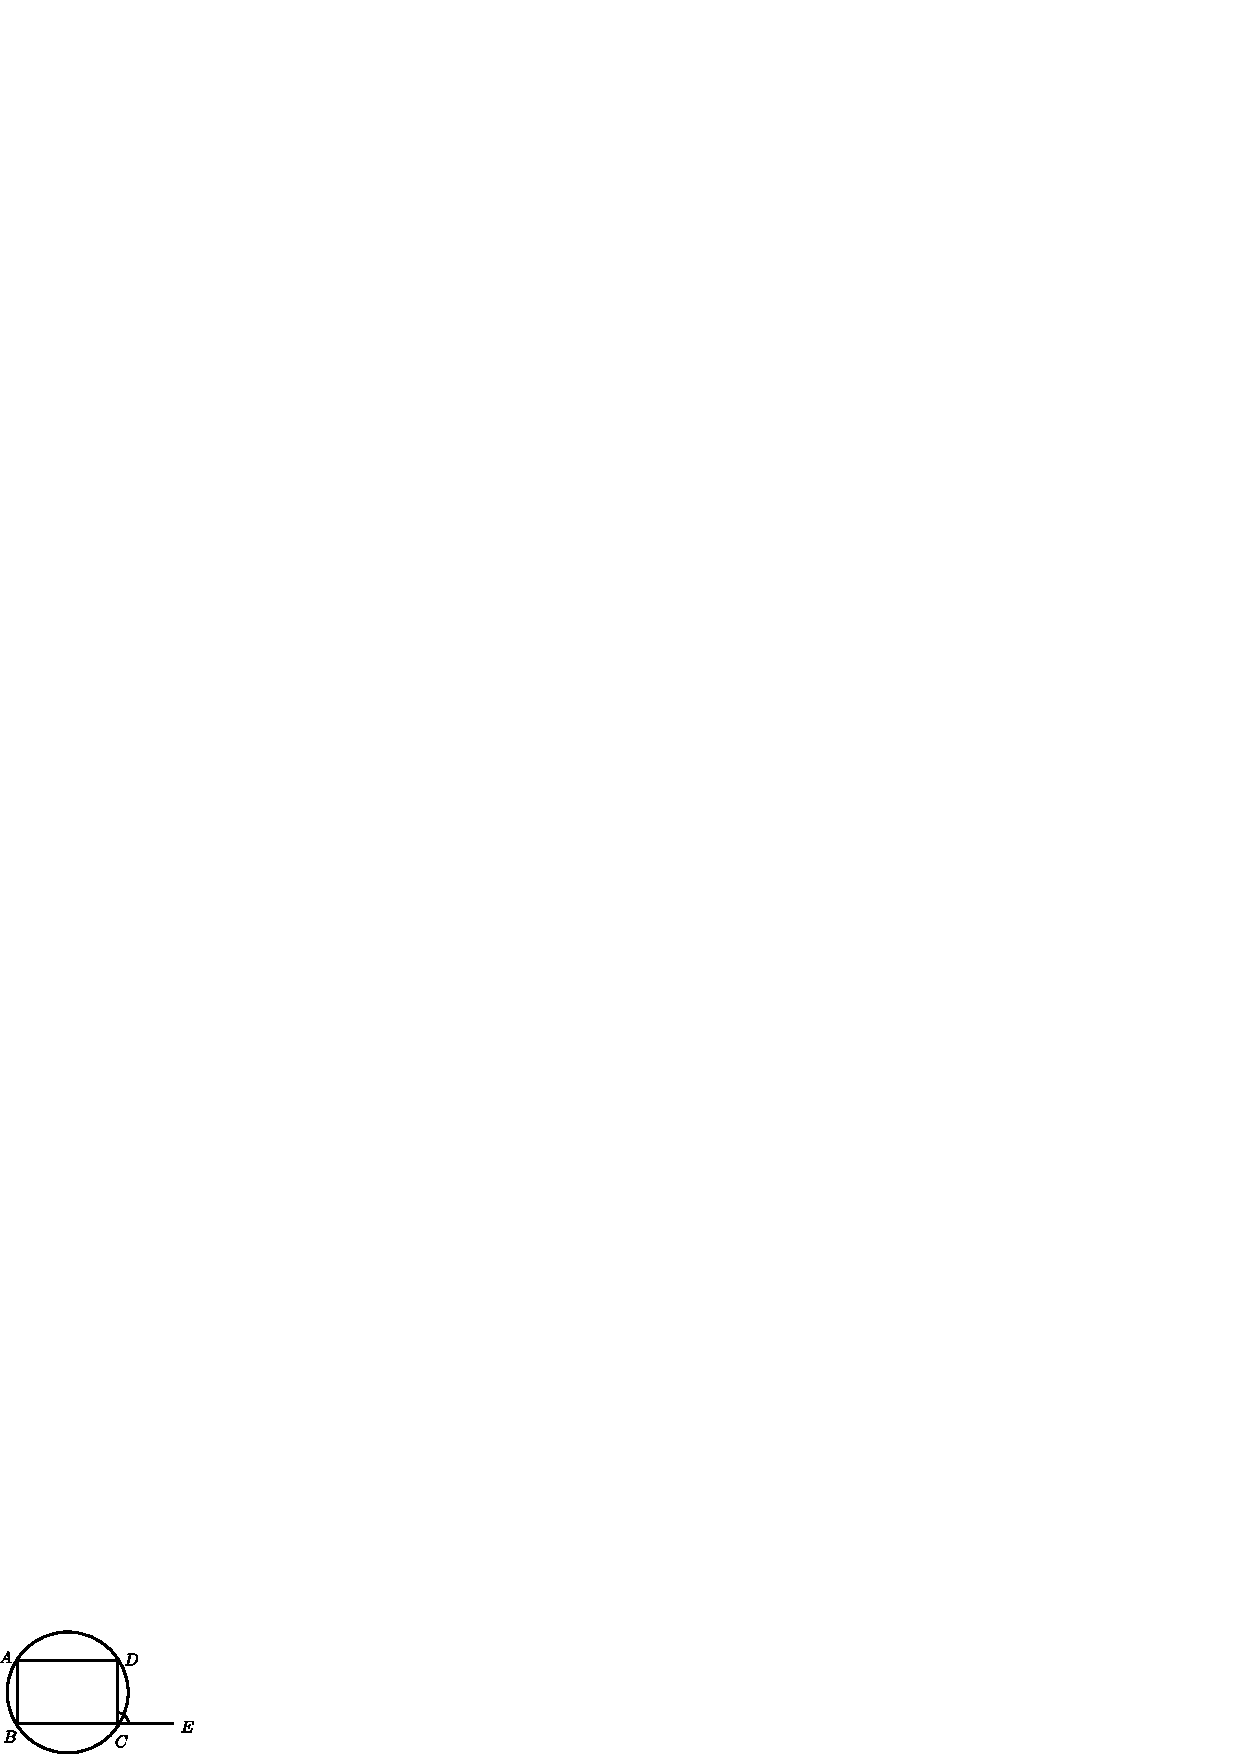
\includegraphics[scale=0.9]{figures/17.png}\\
\textbf{ವಾಕ್ಯಾರ್ಥಗೋಷ್ಠಿಯ ಅಧ್ಯಕ್ಷರಾದ ವಿ. ರಾಜೇಶ್ವರ ಶಾಸ್ತ್ರಿಗಳಿಗೆ ಗೌರ ಪ್ರದಾನ}\\[12pt]
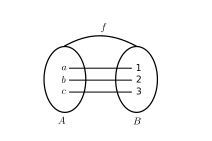
\includegraphics[scale=0.9]{figures/18.png}\\
\textbf{ರಾಜಮಾತೆ ಪ್ರಮೋದಾ ದೇವಿಯವರಿಗೆ ಪೂರ್ಣಕುಂಭ ಸ್ವಾಗತ}\\[12pt]
\includegraphics[scale=0.9]{figures/18a.png}\\
\textbf{ಸಭೆಯೆಡೆಗೆ ಶ್ರೀ ಪಿ.ಎನ್. ಶಾಸ್ತ್ರಿಗಳೊಂದಿಗೆ ರಾಜಮಾತೆ\\ ಪ್ರಮೋದಾ ದೇವಿಯವರ ಶುಭಾಗನ}
\end{tabular}
}

\eject
\thispagestyle{plain}

{\tabcolsep=0pt
\noindent
\begin{tabular}{>{\centering}p{11cm}}
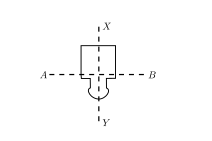
\includegraphics[scale=0.85]{figures/19.png}\\
\textbf{ ಶ್ರೀ ಗಂಗಾಧರ ಭಟ್ಟರು, ಅವರ ಬಲಭಾಗದಲ್ಲಿ ರಾಜಮಾತೆಯವರು, ಅವರ ಪಕ್ಕದಲ್ಲಿ\\ ಶ್ರೀ ಪಿ ಎನ್ ಶಾಸ್ತ್ರಿಗಳು, ಅನಂತರ ಶ್ರೀ ನಿರಂಜನ ವಾನಳ್ಳಿಯವರು, ಪಕ್ಕದಲ್ಲಿ\\ ರಾ.\ ಶಾಸ್ತ್ರಿಗಳು. ಭಟ್ಟರ ಎಡಪಾರ್ಶ್ವದಲ್ಲಿ ಶ್ರೀ ಉಮಾಕಾಂತ ಭಟ್ಟರು}\\[12pt]
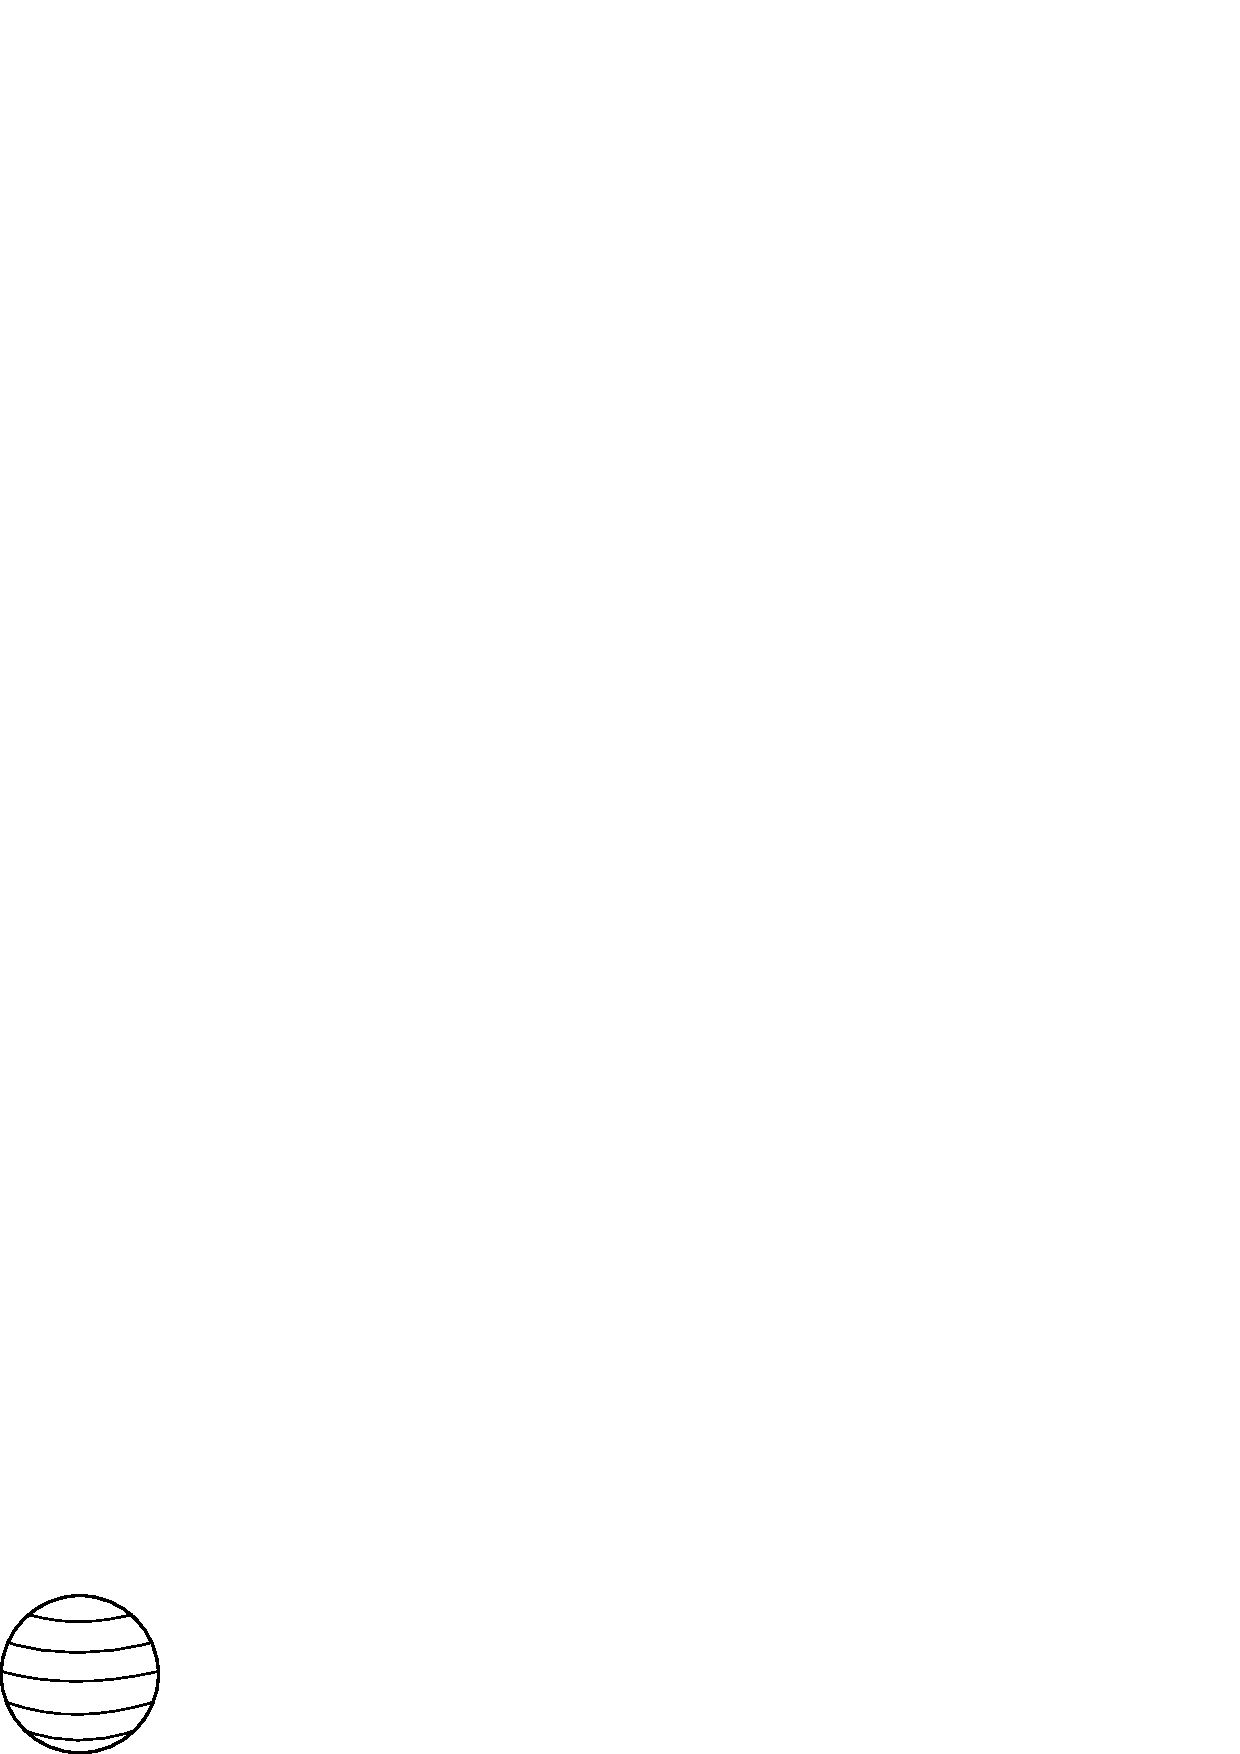
\includegraphics[scale=0.85]{figures/20.png}\\
\textbf{ಸಭೆಯಲ್ಲಿ  ಆಸೀನರಾಗಿರುವ ಅಭಿಮಾನಿ ಸಮೂಹ}\\[12pt]
\includegraphics[scale=0.85]{figures/20a.png}\\
\textbf{ಸಭೆಯಲ್ಲಿ  ಆಸೀನರಾಗಿರುವ ಅಭಿಮಾನಿ ಸಮೂಹ}
\end{tabular}
}

\eject
\thispagestyle{plain}

{\tabcolsep=0pt
\noindent
\begin{tabular}{>{\centering}p{11cm}}
\includegraphics[scale=0.95]{figures/20b.png}\\
\textbf{ಸಭೆಯಲ್ಲಿ  ಆಸೀನರಾಗಿರುವ ಅಭಿಮಾನಿ ಸಮೂಹ}\\[12pt]
\includegraphics[scale=0.95]{figures/20c.png}\\
\textbf{ಸಭೆಯಲ್ಲಿ  ಆಸೀನರಾಗಿರುವ ಅಭಿಮಾನಿ ಸಮೂಹ}\\[12pt]
\includegraphics[scale=0.95]{figures/20d.png}\\
\textbf{ಸಭೆಯಲ್ಲಿ  ಆಸೀನರಾಗಿರುವ ಅಭಿಮಾನಿ ಸಮೂಹ}
\end{tabular}
}

\eject
\thispagestyle{plain}

{\tabcolsep=0pt
\noindent
\begin{tabular}{>{\centering}p{11cm}}
\includegraphics[scale=0.95]{figures/20e.png}\\
\textbf{ಸಭೆಯಲ್ಲಿ  ಆಸೀನರಾಗಿರುವ ಅಭಿಮಾನಿ ಸಮೂಹ}\\[12pt]
\includegraphics[scale=0.95]{figures/20f.png}\\
\textbf{ಸಭೆಯಲ್ಲಿ  ಆಸೀನರಾಗಿರುವ ಅಭಿಮಾನಿ ಸಮೂಹ}\\[12pt]
\includegraphics[scale=0.95]{figures/20g.png}\\
\textbf{ವಿಶಾಲ ಸಭೆ}
\end{tabular}
}

\eject
\thispagestyle{plain}

{\tabcolsep=0pt
\noindent
\begin{tabular}{>{\centering}p{11cm}}
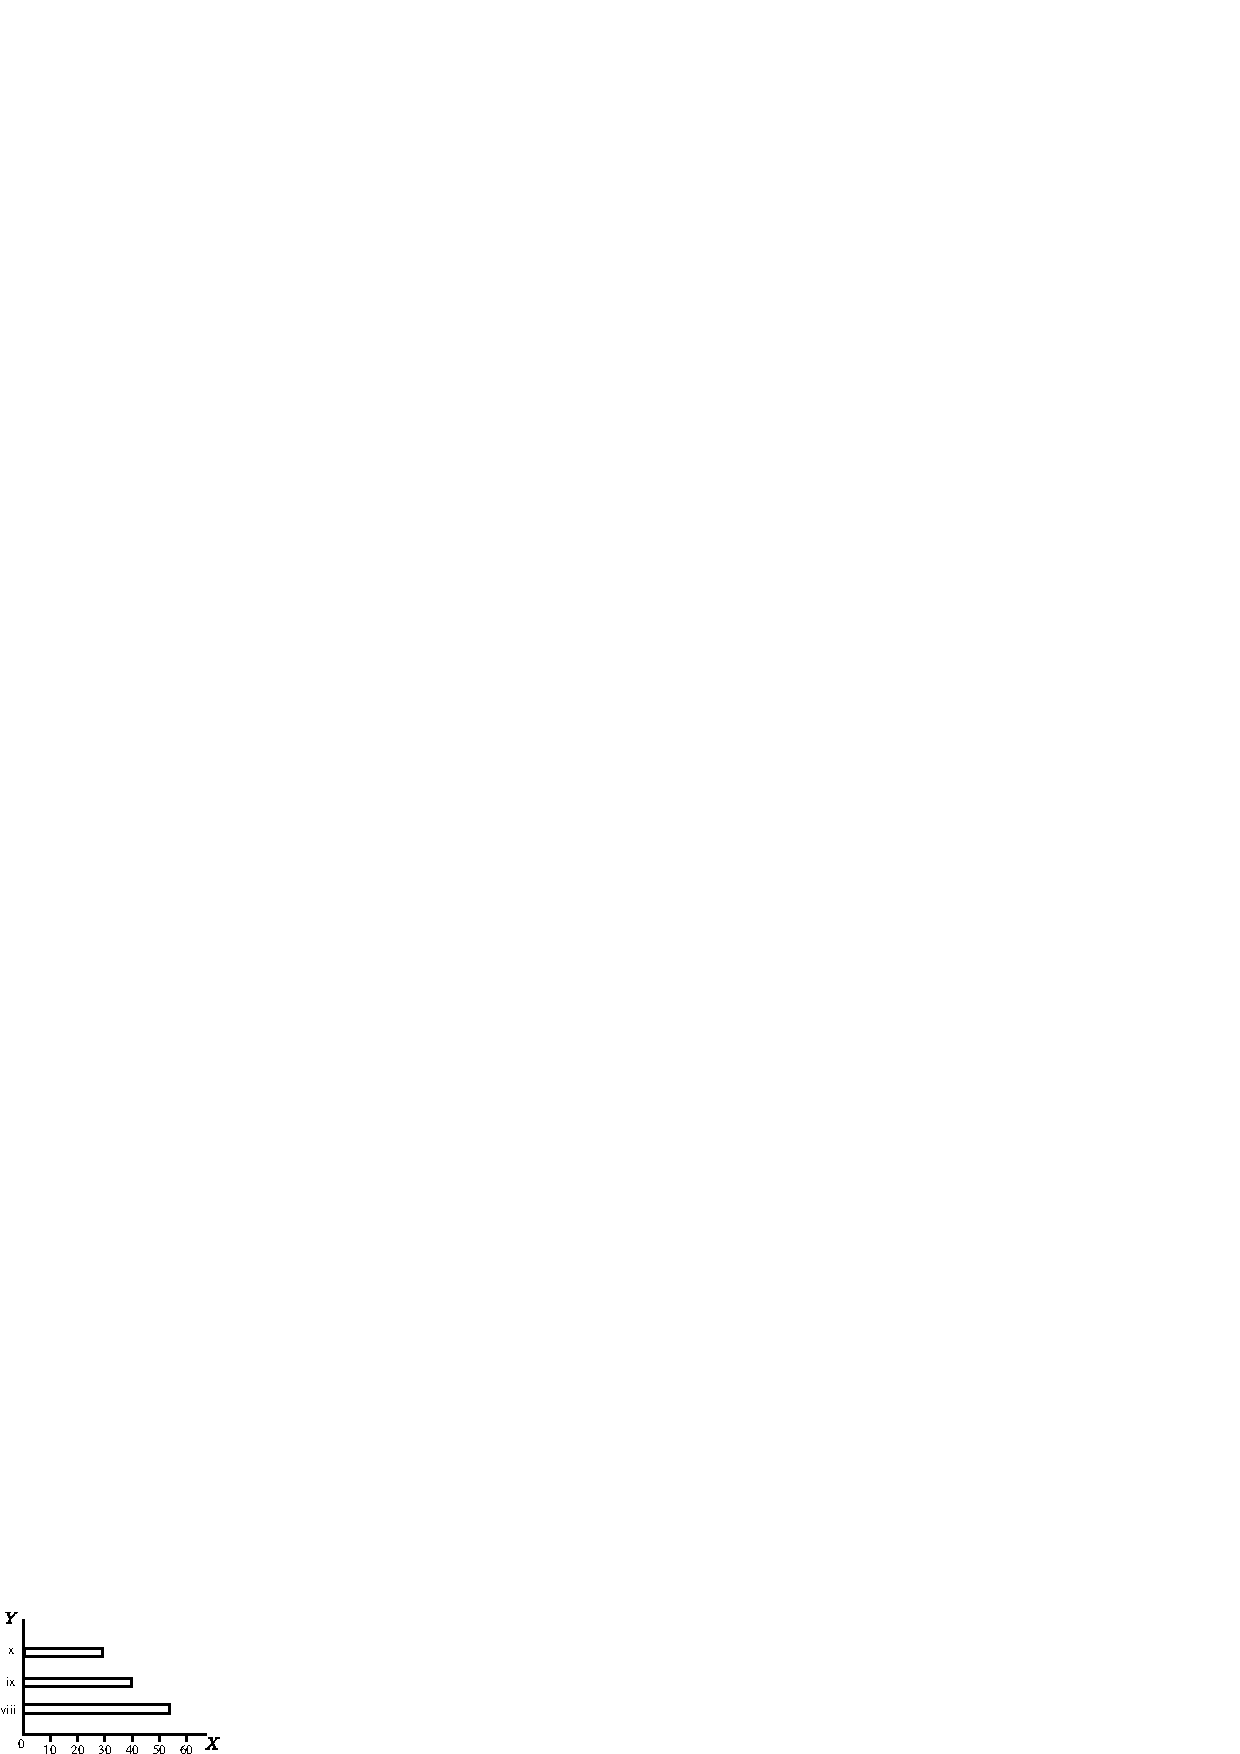
\includegraphics[scale=0.95]{figures/21.png}\\
\textbf{ಸಭಾಸೀನರಾಗಿರುವ ಪಠಶಾಲೆಯ ಅಧ್ಯಾಪಕ ಸಮೂಹ}\\[12pt]
\includegraphics[scale=0.95]{figures/21a.png}\\
\textbf{ಸಭೆಯಲ್ಲಿ  ಆಸೀನರಾಗಿರುವ ಅಭಿಮಾನಿ ಸಮೂಹ}\\[12pt]
\includegraphics[scale=0.95]{figures/22.png}\\
\textbf{ವೇದಸ್ವಸ್ತಿ - ಶ್ರೀ ರಮೇಶ ಅಡಿಗರು ಮತ್ತು ವಿದ್ಯಾರ್ಥಗಳು}
\end{tabular}
}

\eject
\thispagestyle{plain}

{\tabcolsep=0pt
\noindent
\begin{tabular}{>{\centering}p{11cm}}
\includegraphics[scale=0.9]{figures/23.png}\\
\textbf{ಅಭಿವಂದನ ಗ್ರಂಥ ಬಿಡುಗಡೆಯ ಸಂದರ್ಭ}\\[12pt]
\includegraphics[scale=0.9]{figures/23a.png}\\
\textbf{ ಶ್ರೀಗಂಗಾಧರ ಭಟ್ಟರ ಕುರಿತಾದ ಸಾಕ್ಷ್ಯಚಿತ್ರದ\\ ಅನಾವರಣ ರಾಜಮಾತೆ ಪ್ರಮೋದಾ ದೇವಿಯವರಿಂದ}\\[12pt]
\includegraphics[scale=0.9]{figures/24.png}\\
\textbf{ಶ್ರೀಯುತರ ಧರ್ಮಪತ್ನಿ - ಶ್ರೀಮತಿ ಶೈಲಜಾರವರಿಗೆ\\ ಉಡಿತುಂಬಿದ ಶುಭಕ್ಷಣ}
\end{tabular}
}

\eject
\thispagestyle{plain}

{\tabcolsep=0pt
\noindent
\begin{tabular}{>{\centering}p{11cm}}
\includegraphics[scale=0.91]{figures/24a.png}\\
\textbf{ವಿದ್ಯಾರ್ಥಿಗಳು ಸಮರ್ಪಿಸುವ ಸನ್ಮಾನ ಸ್ವೀಕಾರಕ್ಕೆ \\ ಆಸೀನರಾಗಿರುವ ಆಚಾರ್ಯದಂಪತಿಗಳು}\\[12pt]
\includegraphics[scale=0.91]{figures/25a.png}\\
\textbf{ವಿದ್ಯಾರ್ಥಿಗಳ ಕನಸಿನ ಸನ್ಮಾನ ಸಂದರ್ಭ}\\[12pt]
\includegraphics[scale=0.91]{figures/25b.png}\\
\textbf{ವಿದ್ಯಾರ್ಥಿಗಳ ಕನಸಿನ ಸನ್ಮಾನ ಸಂದರ್ಭ }
\end{tabular}
}

\eject
\thispagestyle{plain}

{\tabcolsep=0pt
\noindent
\begin{tabular}{>{\centering}p{11cm}}
\includegraphics[scale=0.93]{figures/25c.png}\\
\textbf{ಸನ್ಮಾನ ಸಂದರ್ಭ}\\[12pt]
\includegraphics[scale=0.93]{figures/25d.png}\\
\textbf{ಸನ್ಮಾನಿತರಾದ ಆಚಾರ್ಯದಂಪತಿಗಳು}\\[12pt]
\includegraphics[scale=0.93]{figures/25e.png}\\
\textbf{ಡಾ . ಪಿ.ಎನ್.ಶಾಸ್ತ್ರಿಗಳು ಮಾತನಾಡುತ್ತಿರುವ ಸಂದರ್ಭ}
\end{tabular}
}

\eject
\thispagestyle{plain}

{\tabcolsep=0pt
\noindent
\begin{tabular}{>{\centering}p{11cm}}
\includegraphics[scale=0.91]{figures/25f.png}\\
\textbf{ಡಾ.ಆಳ್ವಾರ್ ರವರು ಅಧ್ಯಾಪಕ ಸಂಘದ ಪರವಾಗಿ ಮಾತನಾಡುತ್ತಿರುವುದು}\\[12pt]
\includegraphics[scale=0.91]{figures/25g.png}\\
\textbf{ಶ್ರೀಮಾನ್ ಉಮಾಕಾಂತ ಭಟ್ಟರು ಮಾತನಾಡುತ್ತಿರು ಸಂದರ್ಭ}\\[12pt]
\includegraphics[scale=0.91]{figures/25h.png}\\
\textbf{ಸನ್ಮಾನ ಸಂದರ್ಭ - ಶ್ರೀ ಎನ್ ಎಸ್ ರಾಮಭದ್ರಾಚಾರ್ಯರ\\ ಭಾವಚಿತ್ರ ಸಮರ್ಪಣೆ}
\end{tabular}
}

\eject
\thispagestyle{plain}

{\tabcolsep=0pt
\noindent
\begin{tabular}{>{\centering}p{11cm}}
\includegraphics[scale=0.95]{figures/26.png}\\
\textbf{ ಶ್ರೀಯುತರು ಮಾತನಾಡುತ್ತಿರುವ ಸಂದರ್ಭದ}\\[12pt]
\includegraphics[scale=0.95]{figures/26a.png}\\
\textbf{ರಾಜಮಾತೆಯವರು ಮಾತನಾಡುತ್ತಿರುವ ಸಂದರ್ಭ}\\[12pt]
\includegraphics[scale=0.95]{figures/26b.png}\\
\textbf{ರಾಜಮಾತೆ ಪ್ರಮೋದಾದೇವಿಯವರಿಗೆ ಗೌರವ ಸಮರ್ಪಣೆ}
\end{tabular}
}

\eject
\thispagestyle{plain}

{\tabcolsep=0pt
\noindent
\begin{tabular}{>{\centering}p{11cm}}
\includegraphics[scale=0.86]{figures/27.png}\\
\textbf{ಸಭಾಧ್ಯಕ್ಷರಾದ ಶ್ರೀ ನಿರಂಜನ ವಾನಳ್ಳೀಯವರು\\ ಮಾತನಾಡುತ್ತಿರುವ ಸಂದರ್ಭ}\\[12pt]
\includegraphics[scale=0.86]{figures/28.png}\\
\textbf{ಕಾರ್ಯಕ್ರಮದ ಅಂತ್ಯಮಂಗಳ}\\[12pt]
\includegraphics[scale=0.86]{figures/28a.png}\\
\textbf{ಶ್ರೀಗಣಪತಿಸಚ್ಚಿದಾನಂದ ಆಶ್ರಮದ ವತಿಯಿಂದ\\ ಶ್ರೀಯುತರಿಗೆ ಗೌರವ ಸಮರ್ಪಣೆ}
\end{tabular}
}

\eject
\thispagestyle{plain}

{\tabcolsep=0pt
\noindent
\begin{tabular}{>{\centering}p{11cm}}
\includegraphics[scale=0.9]{figures/28b.png}\\
\textbf{ಕಾರ್ಯಕ್ರಮದ ಅಂತ್ಯಮಂಗಳ ಸಂದರ್ಭದಲ್ಲಿ ಸಭೆ}\\[12pt]
\includegraphics[scale=0.9]{figures/29.png}\\
\textbf{ಹವ್ಯಕ ಸಂಘದ ಅಧ್ಯಕ್ಷ ಶ್ರೀ ಲಕ್ಶ್ಮೀನಾರಾಯಣರಿಂದ ಗೌರವಾರ್ಪಣೆ}\\[12pt]
\includegraphics[scale=0.9]{figures/30.png}\\
\textbf{ಸುಧರ್ಮಾದಿಂದ ಗೌರವಾರ್ಪಣೆ - ಸಂಪಾದಕರಾದ ಗೌರವಸಂಪಾದಕರಾದ\\ ಶ್ರೀ ಟಿ.ವಿ. ಸತ್ಯನಾರಾಯಣರವರು ಶ್ರೀ ವಿ.ಡಿ. ಹೆಗಡೆಯವರು}
\end{tabular}
}

\eject
\thispagestyle{plain}

{\tabcolsep=0pt
\noindent
\begin{tabular}{>{\centering}p{11cm}}
\includegraphics[scale=0.92]{figures/31.png}\\
\textbf{ಪ್ರೀತಿಯ ವಿದ್ಯಾರ್ಥಿಸಮೂಹದೊಂದಿಗೆ ಶ್ರೀಗಂಗಾಧರ ಭಟ್ಟರು}\\[12pt]
\includegraphics[scale=0.92]{figures/32.png}\\
\textbf{ಕುಟುಂಬ ವರ್ಗದೊಂದಿಗೆ ಶ್ರೀಯುತರು}\\[12pt]
\includegraphics[scale=0.92]{figures/33.png}\\
\textbf{ ಶ್ರೀ ಭಟ್ಟ್ರರ ಧರ್ಮಪತ್ನಿ - ಶ್ರೀಮತಿ ಶೈಲಜಾರವರ\\ ತವರುಮನೆಯವರೊಂದಿಗೆ ಶ್ರೀಯುತರು}
\end{tabular}
}
\label{prelims_pages}
